\documentclass[convert={outfile=\jobname.svg}]{standalone}
\usepackage[dvipsnames]{xcolor}
\usepackage{tikz}
\usetikzlibrary{calc}
\usetikzlibrary{decorations.pathreplacing,decorations.markings}
\tikzset{dot/.style={draw,shape=circle,fill=black,scale=0.4}}
\tikzset{
  % style to apply some styles to each segment of a path
  on each segment/.style={
    decorate,
    decoration={
      show path construction,
      moveto code={},
      lineto code={
        \path [#1]
        (\tikzinputsegmentfirst) -- (\tikzinputsegmentlast);
      },
      curveto code={
        \path [#1] (\tikzinputsegmentfirst)
        .. controls
        (\tikzinputsegmentsupporta) and (\tikzinputsegmentsupportb)
        ..
        (\tikzinputsegmentlast);
      },
      closepath code={
        \path [#1]
        (\tikzinputsegmentfirst) -- (\tikzinputsegmentlast);
      },
    },
  },
  % style to add an arrow in the middle of a path
  mid arrow/.style={postaction={decorate,decoration={
        markings,
        mark=at position .5 with {\arrow[#1]{stealth}}
      }}},
}

\begin{document}
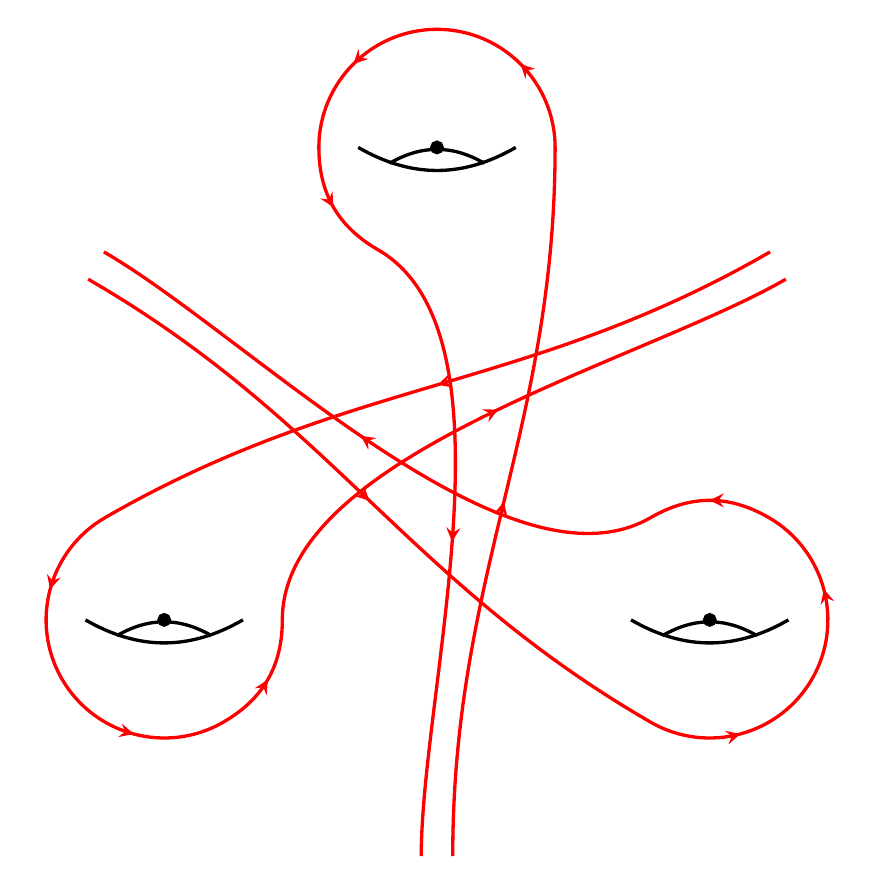
\begin{tikzpicture}[scale=2, very thick]
\foreach \r in {90, 210, 330} {
    \foreach \i in {2} {
    \begin{scope}[shift={(\r:\i)}]
        \draw (-0.5,0) to [out=-30,in=180+30] (0.5,0);
        \draw (-0.3,-0.1) to [out=30,in=180-30] (0.3,-0.1);
    \end{scope}
    }
    \begin{scope}[rotate=\r]
        \node [dot] at (240:2) {};
        \path [draw=red, postaction={on each segment={mid arrow=red}}] ($(60:2.5)+(150:0.1)$)
            to [out=240,in=60] ($(240:2)+(150:0.75)$)
            to [out=240,in=150] ($(240:2)+(240:0.75)$)
            to [out=330,in=240] ($(240:2)+(330:0.75)$)
            to [out=60,in=300] ($(240:2)+(30:0.75)$)
            to [out=120,in=240,looseness=0.7] ($(60:2.5)+(330:0.1)$);
    \end{scope}
}
\end{tikzpicture}
\end{document}
